\documentclass[12pt]{article}

\usepackage{graphicx}
\usepackage{amsmath}
\usepackage{amssymb}
\usepackage{natbib}
\usepackage{amsfonts}
\usepackage{multicol}
\usepackage{float}
\usepackage{oldgerm}
\usepackage{bm}
\usepackage{mathtools}
\usepackage{wrapfig}
\usepackage{fancyhdr}
\usepackage[export]{adjustbox}
\usepackage{xcolor}

\pagestyle{empty}

\newcommand{\Avec}{\mathbf A}
\newcommand{\Bvec}{\mathbf B}
\newcommand{\Dvec}{\mathbf D}
\newcommand{\Evec}{\mathbf E}
\newcommand{\Fvec}{\mathbf F}
\newcommand{\Jvec}{\mathbf J}
\newcommand{\Lvec}{\mathbf L}
\newcommand{\Mvec}{\mathbf M}
\newcommand{\Pvec}{\mathbf P}
\newcommand{\Rvec}{\mathbf R}
\newcommand{\Svec}{\mathbf S}
\newcommand{\Tvec}{\mathbf T}
\newcommand{\avec}{\mathbf a}
\newcommand{\bvec}{\mathbf b}
\newcommand{\dvec}{\mathbf d}
\newcommand{\evec}{\mathbf e}
\newcommand{\fvec}{\mathbf f}
\newcommand{\jvec}{\mathbf j}
\newcommand{\kvec}{\mathbf k}
\newcommand{\nvec}{\mathbf n}
\newcommand{\pvec}{\mathbf p}
\newcommand{\rvec}{\mathbf r}
\newcommand{\svec}{\mathbf s}
\newcommand{\vvec}{\mathbf v}
\newcommand{\xvec}{\mathbf x}
\newcommand{\yvec}{\mathbf y}
\newcommand{\zvec}{\mathbf z}
\newcommand{\nablav}{\boldsymbol{\nabla}}
\newcommand{\nablavector}{\vec \nabla}
\newcommand{\alphavec}{\boldsymbol{\alpha}}
\newcommand{\phivec}{\boldsymbol{\phi}}
\newcommand{\thetavec}{\boldsymbol{\theta}}
\newcommand{\omegavec}{\boldsymbol{\omega}}
\newcommand{\tauvec}{\boldsymbol{\tau}}
\newcommand{\ezero}{\varepsilon_{0}}
\newcommand{\mzero}{\mu_{0}}
\newcommand{\mubold}{\boldsymbol{\mu}}
\newcommand{\uniti}{\hat{\boldsymbol{\imath}}}
\newcommand{\unitj}{\hat{\boldsymbol{\jmath}}}
\newcommand{\unitk}{\hat{\boldsymbol{\mathit{k}}}}
\newcommand{\unitn}{\hat{\mathbf n}}
\newcommand{\unitr}{\hat{\mathbf r}}
\newcommand{\unitphi}{\hat{\boldsymbol{\phi}}}
\newcommand{\unittheta}{\hat{\boldsymbol{\theta}}}

\newcommand{\bit}{\begin{itemize}}
\newcommand{\eit}{\end{itemize}}

\setlength{\headsep}{0.5cm}
\setlength{\oddsidemargin}{-0.5cm}
\setlength{\textwidth}{16.5cm}
\setlength{\textheight}{24cm}
\voffset = -2cm

\pagestyle{fancy}
\fancyhf{}
\rfoot{
\includegraphics[width=1.0in]{cnm.png}}
\lfoot{Homework 11}
\begin{document}

%{\bf \underline{STUDENT NAME}:} 
%\vspace{1cm}

\begin{center}
\hfil
%\begin{wrapfigure}{l}{0.5in} 
%    
\includegraphics[width=0.5in]{cnm.png}
%\end{wrapfigure}
{\large\bf {ENGR 2910-101: Circuit Analysis}}
\hfill Instructor: Leo Silbert \\
Homework 11: 12/01/21 \hfill Due: 12/06/21\\
\hrulefill\\
\end{center}

%{\em Show all your working to ensure you obtain full points. Partial
%  credit will be given for correct algebraic steps if you fail to
%  obtain the correct final answer.}\\

%\newpage


\noindent
{\bf Question 1} [1]

If the voltage ($v$) and current ($i$) through a circuit element are given by:
\begin{align*}
v(t) &= e^{-t/2}\\
i(t) &= e^{-t/2},
\end{align*}
what is the total energy delivered to the element?\\
 
\noindent
(a) 0 J\\
(b) 1 J \\%x\\
(c) $\tfrac{1}{4}$ J\\
(d) $\infty$\\

\noindent
{\bf Question 2} [1]

Compute the power delivered to the circuit shown below.
\begin{figure}[h!]
     \centering
\vspace{-0.2in}
     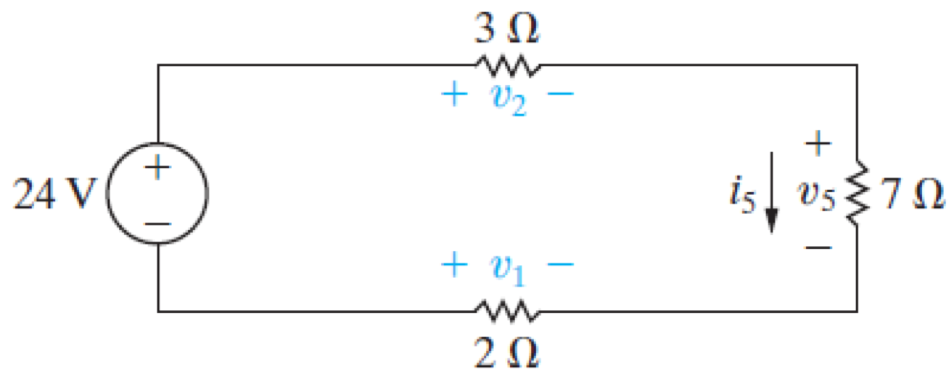
\includegraphics[clip,width=0.4\textwidth]{Fig-AP2-5.png}
\vspace{-0.15in}
\end{figure}

\noindent
(a) 48 W \\%x\\
(b) 12 W\\
(c) 288 W\\
(d) 6 W\\

\noindent
{\bf Question 3} [1]

Find the equivalent resistance for the circuit shown below.
\begin{figure}[h!]
  \centering 
  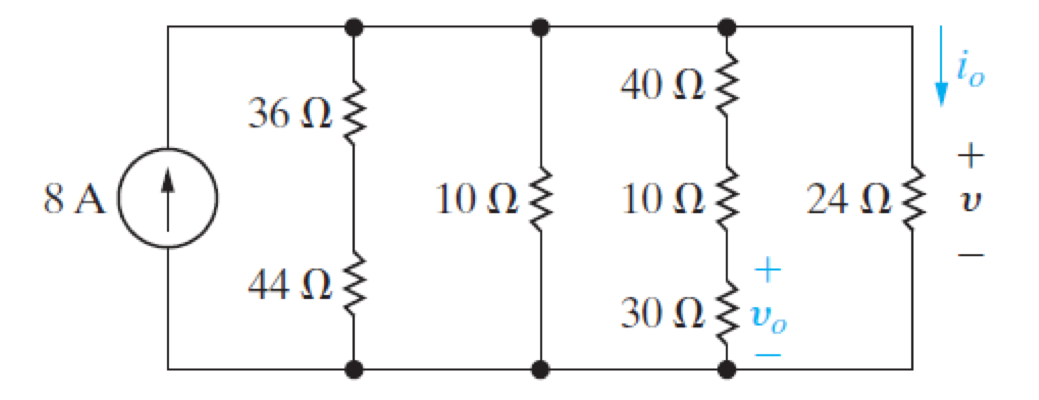
\includegraphics[clip,width=0.6\textwidth]{Fig-E3-7.png}
\end{figure}

\noindent
(a) 6 $\Omega$ \\%x\\
(b) 18 $\Omega$\\
(c) 24 $\Omega$\\
(d) 44 $\Omega$\\

\newpage
\noindent
{\bf Question 4} [1]

For the following circuit find the sum of the voltages ${\color{cyan} v1}$ and ${\color{cyan} v2}$.
\begin{figure}[h!]
  \centering 
  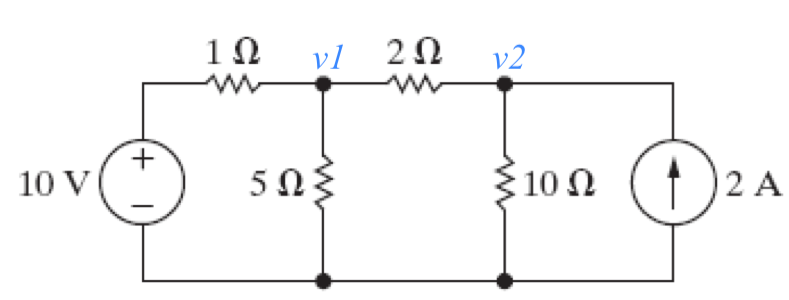
\includegraphics[clip,width=0.55\textwidth]{Fig4-5.png}
\end{figure}

\noindent
(a) 10 V\\
(b) 9 V\\
(c) 20 V \\%x\\
(d) 5 V\\

\noindent
{\bf Question 5} [1]

What is the value of ${\color{cyan} i_{3}}$ in the circuit shown below?
\begin{figure}[h!]
\centering 
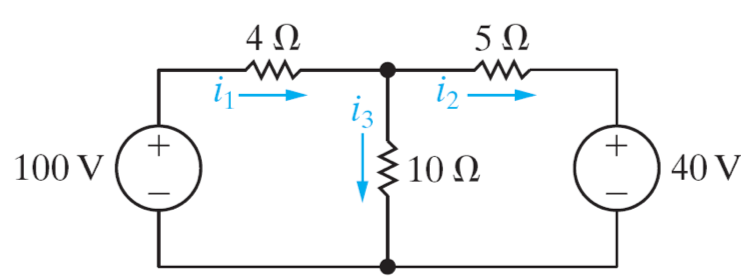
\includegraphics[clip,width=0.5\textwidth]{Fig4-19.png}
\end{figure}

\noindent
(a) 10 A\\
(b) 4 A\\
(c) 14 A\\
(d) 6 A \\%x\\

\noindent
{\bf Question 6} [1]

For $ t > 0$, the current source generates a current, $i = 10 t e^{-5t}$ A, in the circuit shown below. 
\begin{figure}[h!]
\centering 
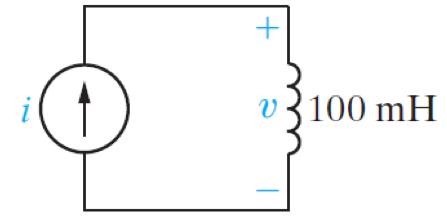
\includegraphics[clip,width=0.3\textwidth]{Fig6-1.png}
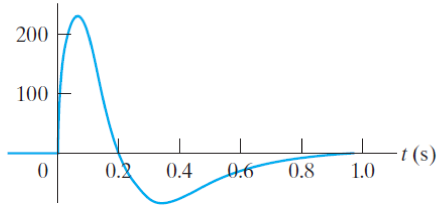
\includegraphics[clip,width=0.4\textwidth]{Fig6-8p.png}
\end{figure}

What does the corresponding graph show?\\

\noindent
(a) Power \\%x\\
(b) Energy\\
(c) Current\\
(d) Voltage\\

\newpage
\noindent
{\bf Question 7} [1]

What is the value of the time constant for the RL circuit shown below?
\begin{figure}[h!]
\centering 
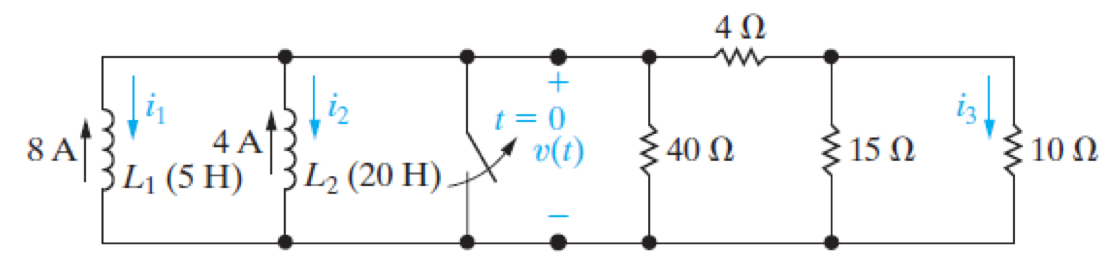
\includegraphics[clip,width=0.8\textwidth]{Fig7-10.png}
\end{figure}

\noindent
(a) 0.590 s\\
(b) 3.125 s\\
(c) 0.500 s \\%x\\
(d) 0.333 s\\

\noindent
\noindent
{\bf Question 8} [1]

Consider a parallel RLC circuit. If, $R = 150 \Omega$, $L = 50$ mH, and $C = 0.2 \mu$F, is the circuit:

\noindent
(a) Critically Damped\\
(b) Overdamped \\%x\\
(c) Underdamped\\

\noindent
\noindent
{\bf Question 9} [1]

Consider a parallel RLC circuit. If, $R = 250 \Omega$, $L = 50$ mH, and $C = 0.2 \mu$F, is the circuit:

\noindent
(a) Critically Damped \\%x\\
(b) Overdamped\\
(c) Underdamped\\

\noindent
\noindent
{\bf Question 10} [1]

Consider a parallel RLC circuit. If, $R = 350 \Omega$, $L = 50$ mH, and $C = 0.2 \mu$F, is the circuit:

\noindent
(a) Critically Damped\\
(b) Overdamped\\
(c) Underdamped \\%x\\


\end{document}
